

\begin{figure}[h!] 
\centering
  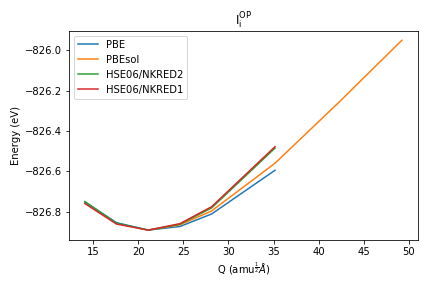
\includegraphics[width=0.7\columnwidth]{figures/ch6/neutral_comparison.png}
  \caption[Potential energy surface of $\mathrm{I}_\mathrm{i}$ calculated at various levels of theory]{Potential energy surface of the neutral iodine interstitial calculated at various levels of theory: GGA (PBE and PBEsol functionals) without spin-orbit coupling and hybrid (HSE06) with spin-orbit coupling. The hybrid wavefunctions have been converged using a single point calculation at the gamma point for the Fock exchange (NKRED=2) or using a $2\!\times\!2\!\times\!2$ Monkhorst-Pack mesh (NKRED=1).}
\end{figure}

\begin{figure}[h!]  
\centering
  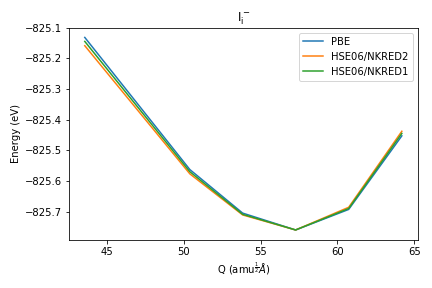
\includegraphics[width=0.7\columnwidth]{figures/ch6/negative_comparison.png}
  \caption[Potential energy surface of $\mathrm{I}_\mathrm{i}^-$ calculated at various levels of theory]{Potential energy surface of the negative iodine interstitial calculated at various levels of theory: GGA (PBE and PBEsol functionals) without spin-orbit coupling and hybrid (HSE06) with spin-orbit coupling. The hybrid wavefunctions have been converged using a single point calculation at the gamma point for the Fock exchange (NKRED=2) or using a $2\!\times\!2\!\times\!2$ Monkhorst-Pack mesh (NKRED=1).}
\end{figure}

\begin{figure}[h!]   
\centering
  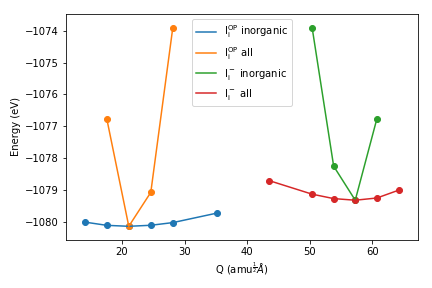
\includegraphics[width=0.7\columnwidth]{figures/ap9/organic_inorganic.png}
  \caption[Potential energy surfaces for all-atom or inorganic-only lattice distortions]{Potential energy surfaces for all-atom or inorganic-only lattice distortions. In Chapter 6 the configuration coordinate $Q$ is defined as $\sqrt{\sum_i m_i \nabla r_i^2}$ ,where the sum is over all inorganic atoms $i$ with mass $m_i$ and a displacement from equilibrium of $\nabla r_i$. As shown in this figure, summing over all atoms, including those in the organic methylammonium molecule, leads to unphysical energies as the linear interpolation does not capture the rotation of the organic cation between charge states.}
\label{schrodinger}
\end{figure}
